
%Taken from aspect manual. 
The SolCx benchmark is intended to test the accuracy of the solution to a problem that 
has a large jump in the viscosity along a line through the domain. Such situations are 
common in geophysics: for example, the viscosity in a cold, subducting slab is much larger 
than in the surrounding, relatively hot mantle material.

The SolCx benchmark computes the Stokes flow field of a fluid driven by spatial density 
variations, subject to a spatially variable viscosity. Specifically, the domain 
is $\Omega = [0,1]^2$, gravity is $\vec{g} = (0,-1)^T$ and the density is given by 
\begin{equation}
\rho(x,y) = \sin(\pi y) \cos(\pi x)
\end{equation}
Boundary conditions are free slip on all of the sides of the domain and the 
temperature plays no role in this benchmark. 
The viscosity is prescribed as follows:
\begin{equation}
\eta(x,y) = 
\left\{
\begin{array}{lll}
1 & \text{for} & x<0.5 \\
10^6 & \text{for} & x>0.5 \\
\end{array}
\right.
\end{equation}
Note the strongly discontinuous viscosity field yields a stagnant flow 
in the right half of the domain and thereby yields a pressure discontinuity along the interface. 

The SolCx benchmark was previously showcased in Duretz \etal (2011) \cite{dumg11} 
and its analytic solution is given in Zhong (1996) \cite{zhon96}. 
It has been carried out in Kronbichler \etal (2012) \cite{krhb12} and Gerya \etal (2013) \cite{gemd13}, 
and is also found in the \aspect manual \cite{aspectmanual}. 

Note that the source code which evaluates the velocity and pressure fields for both SolCx and SolKz is 
distributed as part of the open source package Underworld 
(Moresi \etal, 2007 \cite{moql07}, http://underworldproject.org).
I have translated this code to python. 

\begin{center}
a)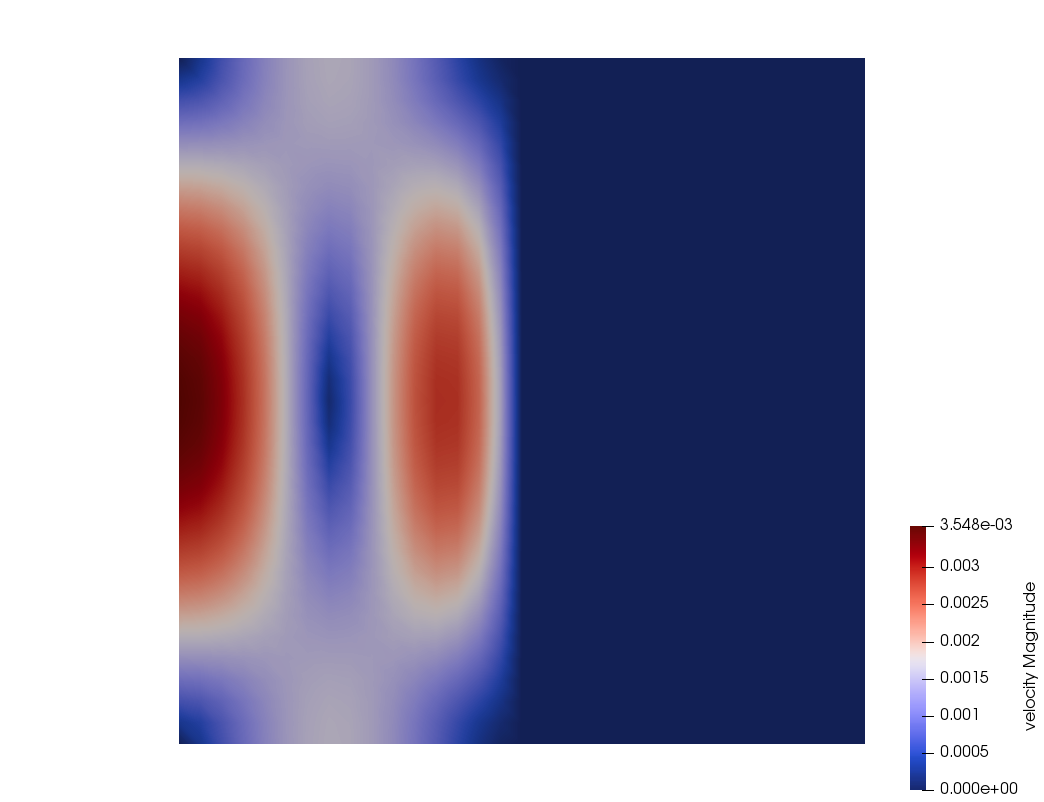
\includegraphics[width=5cm]{images/benchmark_solcx/vel}
b)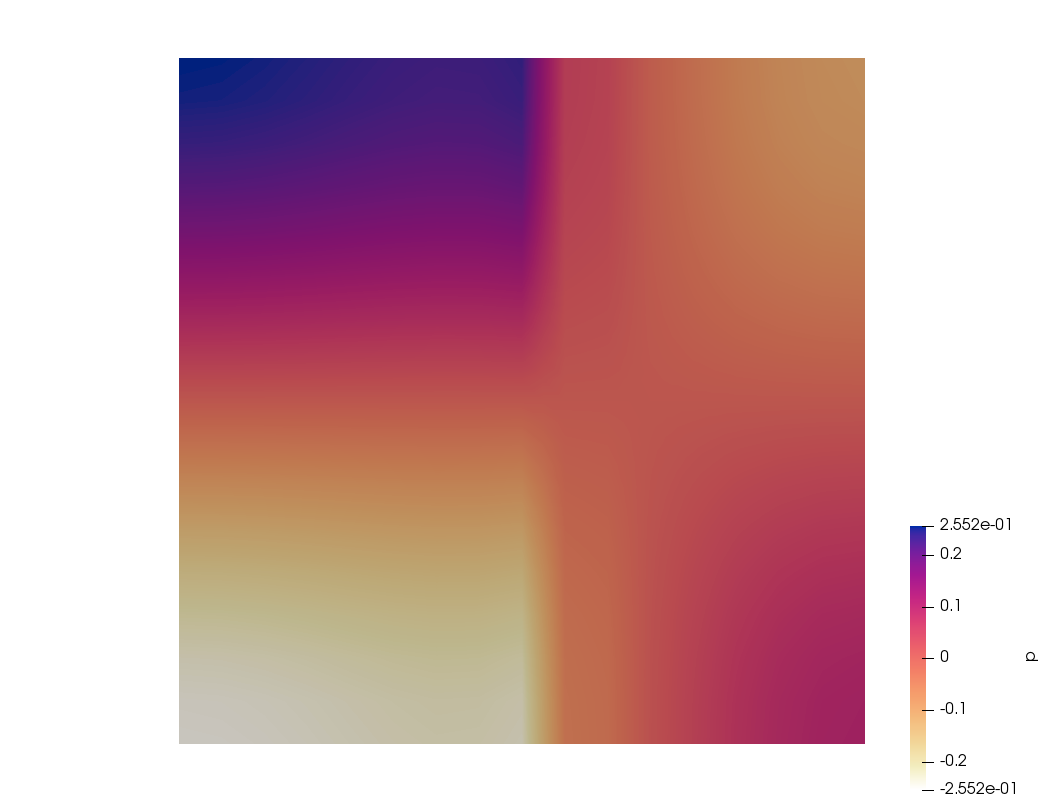
\includegraphics[width=5cm]{images/benchmark_solcx/press}\\
c)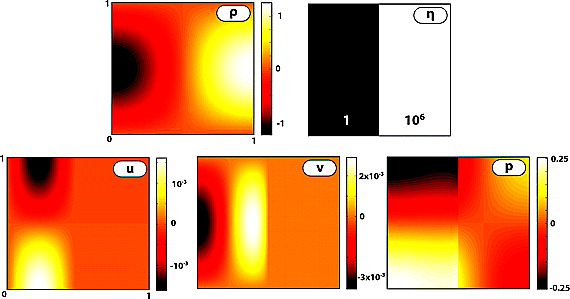
\includegraphics[width=10cm]{images/benchmark_solcx/dumg11}\\
{\captionfont a,b) obtained with \aspect. c) taken from Duretz \etal (2011) \cite{dumg11}.}
\end{center}

\begin{center}
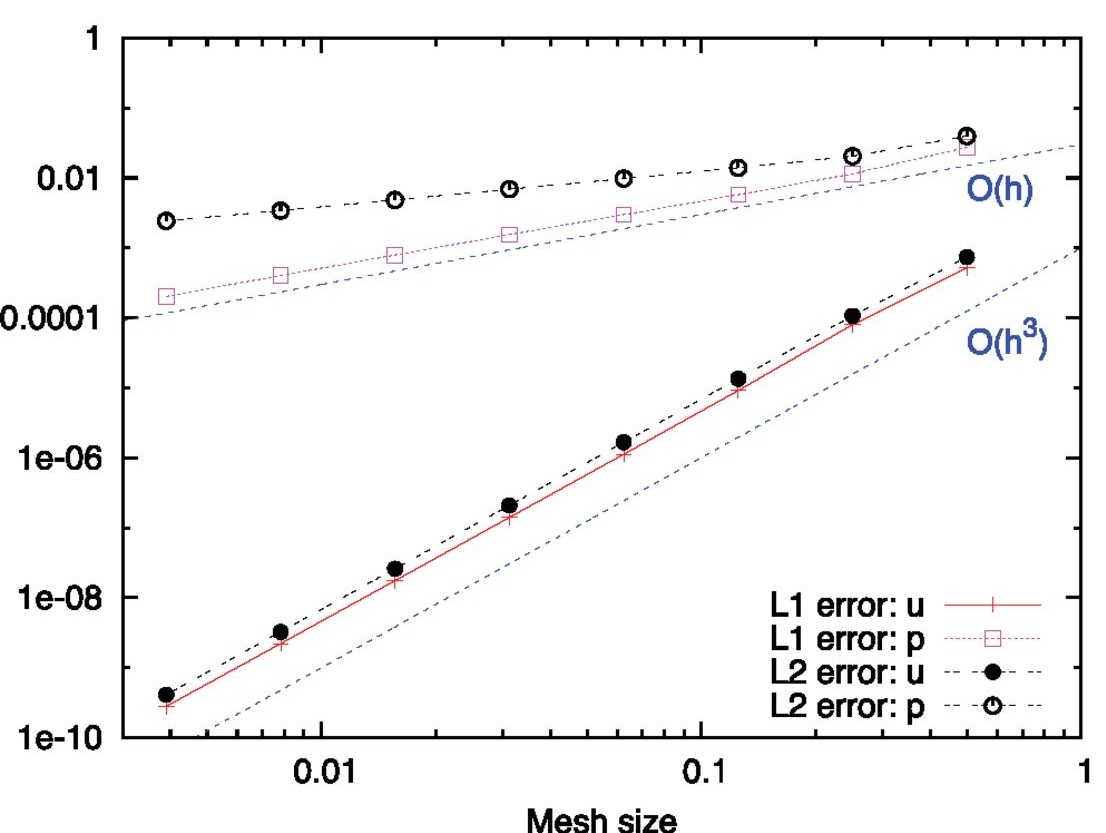
\includegraphics[width=5cm]{images/benchmark_solcx/krhb12}
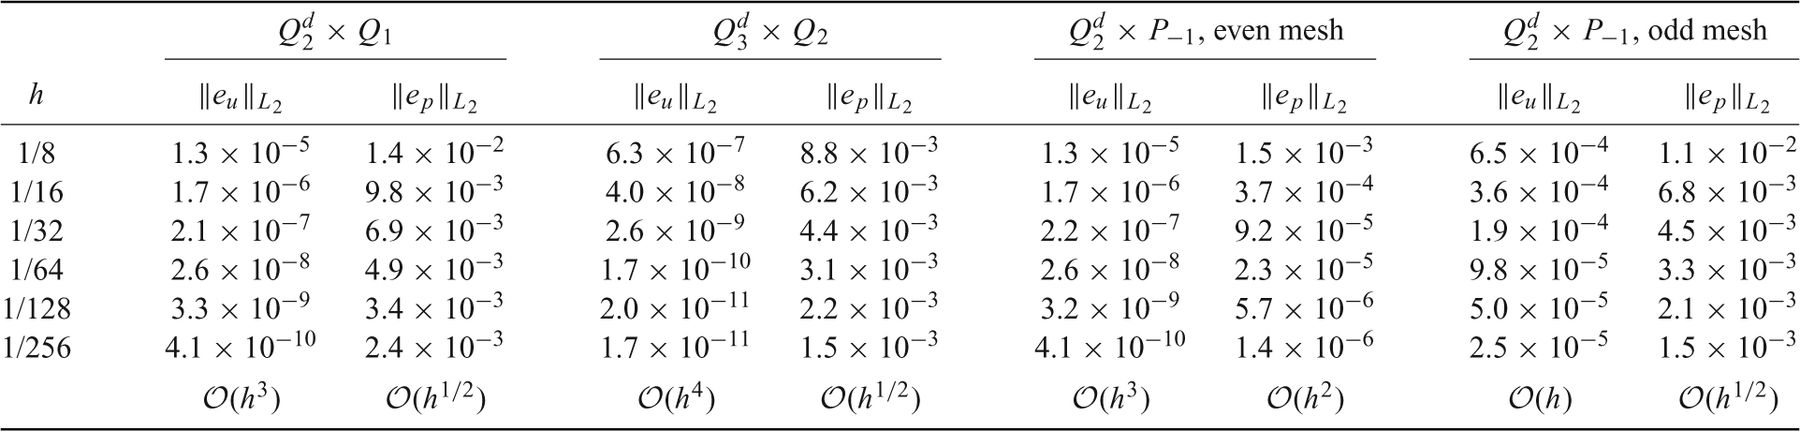
\includegraphics[width=11cm]{images/benchmark_solcx/krhb12b}\\
{\captionfont Taken from Kronbichler \etal (2012) \cite{krhb12}.
Velocity and pressure errors eu, ep and convergence rates for different choices of 
the Stokes finite element spaces, using globally refined meshes. 
For ‘odd’ meshes, the numbers shown are the average errors from nearby meshes 
(e.g. for $h=1/64$, the average of the errors on 63x63 and 65x65 meshes).}
\end{center}


\Literature: \cite{mamo08,vemmXX,demh19} 

\stones 5, 77



